\providecommand{\topdir}{..}
\documentclass[../main.tex]{subfiles}

\ifSubfilesClassLoaded{
  \externaldocument[main-]{../main}
  \setcounterref{chapter}{main-chap:conclusion}
  \addtocounter{chapter}{-1}
}{}

\externaldocument{\subfix{../00_front_matter/front_matter}}
\externaldocument{\subfix{../01_introduction/introduction}}
\externaldocument{\subfix{../02_lorenz96/lorenz96}}
\externaldocument{\subfix{../03_rayleigh_benard/rayleigh_benard}}
\externaldocument{\subfix{../04_tendencies/tendencies}}
\externaldocument{\subfix{../05_evaluation/evaluation}}
\externaldocument{\subfix{../07_appendix/appendix}}

\begin{document}

\ifSubfilesClassLoaded{
    \frontmatter
    \tableofcontents
    \mainmatter
}{}

\chapter{Discussion} \label{chap:conclusion}
\setlength{\epigraphwidth}{.45\textwidth}
\epigraphhead[0.1\textheight]{
    \epigraph{
        God does not care about our mathematical difficulties; He integrates
        empirically.
    }{
        Albert Einstein, quoted by Leopold Infeld in
        \emph{Quest: an autobiography}, 1941
    }
}
\todo{introductory paragraph}
% In \crefrange{chap:rayleigh_benard}{chap:evaluation}, I presented a
% complete proof of concept for data-driven parametrisation in \rb{} convection,
% from the initial formulation of the problem to the assessment of the
% parametrised model in an online setting. In the final chapter of this thesis, I
% will discuss in greater detail the main obstacles that were encountered in the
% process (\cref{sec:issues}) and the concrete outcomes of this work
% (\cref{sec:outcomes}) before drawing final conclusions in
% \cref{sec:conclusion}.


% \section{Practical issues and their implications} \label{sec:issues}
% This work has highlighted several obstacles to the practical implementation
% data-driven parametrisation that were initially not obvious from a purely
% theoretical point of view or not applicable to earlier work using simpler
% dynamical systems such as Lorenz '96. Fundamentally, many of these arise
% because the \rb{} problem is spatially continous---a PDE, as opposed to ODEs
% like Lorenz '96.


\section{Preventing coarse model instability}
One of the earliest issues encountered in this work was the potential for
low-resolution models to become numerically unstable, making it difficult to
obtain a baseline for evaluating parametrised models. Aside from the need for
a baseline, it seems unlikely that a simple parametrisation scheme like the one
developed in \cref{chap:tendencies} would have improved the skill of a
coarse model on the brink of instability. Since this work was not concerned
with accurately representing physical reality, I chose to artificially add
hyperviscosity terms to the equations. Another option for future work could be
to use stress-free boundary conditions on the top and bottom plates (i.e.,
$w(z=0,1) = \partial u/\partial z|_{z=0,1} = 0$) rather than the no-slip
condition. This could reduce the large near-wall temperature and velocity
gradients that often triggered instability at low resolutions.

However, when modelling real-world systems such as the atmosphere, one does
not have the freedom to simply alter the governing equations. Successful
data-driven parametrisation in these cases will depend on the careful choice of
the numerical methods used to discretise and solve the equations such that
the underlying coarse model is stable, even if it is inaccurate. Futher work
with the \rb{} system should investigate whether other types of solvers
(finite difference/volume/element, etc.) are more suitable.


\section{The coarse-graining problem}
\todo{move to conclusion}

The predictability of the subgrid tendencies was found to depend strongly on
the method used to coarse-grain the high-resolution solutions, and the
development of an an appropriate method was non-trivial. These findings
can be justified with further discussion.

The Lorenz '96 system \cref{eqn:l96} explicitly separates its degrees of
freedom into ``coarse'' and ``fine'' variables, allowing one to unambiguously
define a reduced model by simply truncating the fine variables from the full
model. The corresponding ``coarse-graining'' operation is trivial: just discard
the fine variables. For spatially continuous systems like \rb{}, however,
standard practice is to construct high- and low-resolution models independently
from each other by applying (possibly different) discretisation schemes to the
governing equations. Since the low-resolution model is not, in general,
obtained by explicitly truncating the high-resolution model, it is up to the
modeller to choose a coarse-graining operation that maps the high-resolution
state space to the low-resolution one. While instructive, Lorenz '96 and its
coarse/fine paradigm are not helpful analogues in this respect.


\section{Strategies for improving subgrid tendency prediction}
\label{sec:improve_prediction}
% § Alternative approaches in literature (Alieva, Gentine papers)
Another obstacle to data-driven parametrisation for spatially continuous
problems is that there is a very large number of possible subgrid tendency
predictors. For \rb{}, one not only has the three prognostic variables, but
also their derivatives to arbitrary order in the two spatial directions. The
position-dependence of the subgrid tendency statistics was a further
complication, adding $z$ to the list of predictors. One could even use
spatially or temporally nonlocal predictors (i.e., the values of the variables
at nearby points in space or previous time steps)---a possibility that was not
even considered in this work. It would be impossible for a human to explore
every possible combination. Supervised machine learning algorithms, discussed
briefly in \cref{sec:data_driven}, are much better-suited to regression
problems with large numbers of predictors and could potentially capture hidden
and/or nonlinear relationships between these predictors and the subgrid
tendencies. There is no doubt, however, that this work was limited by the
simplicity of the predictors and regression models that were considered, and
future work using more sophisticated statistical models may indeed have greater
success without needing to resort to machine learning.

This work was further limited by its use of purely deterministic
parametrisation schemes despite the existence of considerable residuals
in the subgrid tendency regressions
\crefrange{fig:theta_subgrid_vs_pred_tend}{%
fig:w_subgrid_vs_pred_tend}. Stochastic parametrisation, discussed in
\cref{sec:stochastic}, has the potential to reduce mean-state model
biases by emulating the observed residuals. With the tools I have developed for
the \rb{} problem, it would be relatively straightforward to experiment with
various stochastic perturbations of the existing deterministic scheme
\cref{eqn:scheme}, beginning with those that have been tested for
Lorenz '96 (see \cref{sec:l96_statmodels}). This would include the use
of time-correlated (e.g., AR(1)) noise to reflect the persistence (memory)
of the subgrid tendencies.


\section{Physical explanation of subgrid tendency correlations}
\label{sec:tendency_explanation}
% ○ There is evidence that subgrid tendencies are still predictable from the large-scale state
% ○ Resolved tendency correlation
%   § Insufficient dissipation - paper
%   § Convection causes converging moisture to rain out
Despite the difficulties described in \cref{sec:improve_prediction}, the joint
histograms in \cref{chap:tendencies} gave clear evidence of subgrid tendency
predictability in the near-wall regions. In this section, I argue that
(at least) the correlations involving the $\theta$ subgrid tendency can
be physically explained and are not spurious. As a reminder, the results in
question are:
\begin{enumerate}
    \item The negative correlation between the $\theta$ subgrid tendency and
        $w$ near $z=0,1$,
    \item The positive correlation between the $\theta$ subgrid tendency and
        $\partial u/\partial x$ near $z=0$ and the negative correlation near
        $z=1$, and
    \item The negative correlation between the $\theta$ subgrid tendency and
        the $\theta$ tendency predicted by the coarse model, near $z=0,1$.
\end{enumerate}

I attribute these to the coarse-graining step, which, in the process of
smoothing the temperature field, widens the thermal boundary layer considerably
(compare \cref{fig:coarse_graining_example}a to
\cref{fig:coarse_graining_example}c). On the one hand, there is little change
in boundary layer thickness between the coarse state at time $t$ and the true
coarse state at time $t + \delta t$ because the latter is obtained by first
applying the fine model to the fine state at time $t$ (\cref{itm:fine_model})
and then coarse-graining (\cref{itm:coarse_grain}). This means that the true
coarse tendencies (\cref{itm:true_tend}) are close to zero in the boundary
layers. On the other hand, the coarse model prediction for time $t + \Delta t$
is obtained by first coarse-graining the fine state at time $t$
(\cref{itm:coarse_grain}) and \emph{then} applying the coarse model
(\cref{itm:coarse_model}). At the high Rayleigh number used here ($\rayleigh =
10^9$), advection in the coarse model immediately begins to thin out the
unusually thick boundary layers.

\cref{fig:tendency_explanation} gives a cartoon illustration of the effect of
advection on the temperature field. Consider the bottom left green dot,
which is located near the lower wall, at the base of a rising convection
plume. At this point, the vertical velocity $w$ is positive, and fluid is
rushing inwards from the left and right, making $\partial u/\partial x$
negative. The aforementioned widening of the thermal boundary layer by
the coarse-graining operation has effectively created a large mass of warmer
fluid beneath; this is advected upwards in the coarse model, meaning that
the coarse model predicts a positive tendency $\partial\theta/\partial t$
at the green dot. As explained in the previous paragraph, the true value of
$\partial\theta/\partial t$ is closer  to zero at this point. The subgrid
tendency---the true tendency minus predicted tendency---is therefore negative.

Applying the same logic to the other three green dots in
\cref{fig:tendency_explanation}, as shown by the text boxes, one finds that the
signs of $w$ and the predicted tendency are always opposite to the sign of the
subgrid tendency. The conclusion is that these variables must be negatively
correlated with the subgrid tendency near $z=0,1$. On the other hand, the
$\partial u/\partial x$ has the same sign as the subgrid tendency near $z=0$
(i.e., positive correlation) and the opposite sign near $z=1$ (i.e., negative
correlation). These predictions are all consistent with the observations in
\cref{chap:tendencies}.

It is farily easy to attribute the subgrid $\theta$ tendency correlations to
advection in the coarse model because $\theta$ behaves a tracer that is nearly
conserved by the flow. The velocity field, however, also has a boundary layer
that is widened by the coarse-graining operation, leading me to conjecture that
the subgrid $u$ and $w$ tendency correlations can be explained using a similar
argument. The fact that all the correlations exhibit similar height dependence
lends credence to the conjecture. If this is true, then the fact that $\theta$
is more closely conserved by the flow than $u$ or $w$ could explain why the
correlations for $\theta$ were observed to be consistenly stronger than the
other variables (see, e.g., \cref{tab:r_squared}).

\begin{figure}[ht]
    \centering
    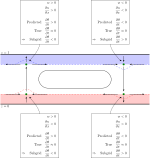
\includegraphics[width=0.8\linewidth]{figures/tendency_explanation.pdf}
    \caption{
        Cartoon illustration of the effect of advection on the coarse-grained
        temperature field when it is evolved using the coarse model. Thick
        horizontal black lines represent the top and bottom domain walls. Black
        arrows represent the velocity field. The warm and cold thermal boundary
        layers are indicated by red and blue shading respectively. Advection
        deforms the isotherms in the boundary layer, which are initially
        approximately flat, in the manner indicated by the dashed red and blue
        lines. The text boxes list the signs of the predictors and predictands
        at the four green dots, demonstrating the claimed correlations.
    }
    \label{fig:tendency_explanation}
\end{figure}

While it is not surprising that the subgrid tendency statistics are
height-dependent, it is interesting that this work was unable to produce
evidence of predictability in the interior of the domain, away from $z=0,1$.
Future work should investigate whether more advanced statistical models and/or
machine learning are able to reveal correlations in this region.


\section{Unanswered questions}
% ○ Address goals that were not achieved, how they might be addressed using tools developed here
% § Assess value added by stochasticity and memory
%     ○ And the way in which they are added - e.g. additive vs. multiplicative noise, spatially/temporally correlated vs. white noise
% § Relationship between offline correlation and online performance
% § Relationship between short-term forecast skill and long-term statistics (refer to results)

% refer to framework/tools
% § Reproducibility, readability
% § Capabilities


\section{Conclusion} \label{sec:conclusion}
% ○ Developed an understanding of the practical issues involved in data-driven parametrisation
% ○ Methods from L96 do not easily generalise to real fluid models
% ○ Successful proof of concept and concrete tools for further research
% § Data-driven works

% much to be learned

\ifSubfilesClassLoaded{%
    \emergencystretch=5em
    \printbibliography{}
}{}

\end{document}
